\documentclass[a4paper,11pt,twoside]{report}

\usepackage[default]{lato}
\usepackage{setspace}
\usepackage[T1]{fontenc}
\usepackage[]{algorithm2e}
\usepackage[latin1]{inputenc}
\usepackage[english,german]{babel}
\usepackage{graphicx,float,latexsym,textcomp,longtable,verbatim,dsfont}
\usepackage{abstract}
\usepackage{epsfig}
\usepackage{amssymb}
\usepackage{amsmath}
\usepackage{amsfonts}
\usepackage{ragged2e}
\usepackage{caption}
\usepackage{hyperref}
\usepackage{microtype}
\usepackage[section]{placeins}
\usepackage[authoryear]{natbib}


\captionsetup[table]{skip=10pt}
\pdfmapfile{+lato.map}

\graphicspath{{./gfx/}}

\setlength{\oddsidemargin}{1cm}
\setlength{\evensidemargin}{0cm}
\setlength{\textwidth}{15cm}



\newcommand{\titel}{Biologically Inspired Model for Coding Sensorimotor Experience Leading to the Development of Pointing Behaviour in a Humanoid Robot}
\newcommand{\ssom}{$5\times5$ }
\newcommand{\bsom}{$15\times15$ }


\begin{document}
\selectlanguage{english}
\onehalfspacing
\begin{titlepage}
\hspace{10cm}
\vspace{4cm}

\begin{center}
  \vspace{-4 cm}
  \huge{\bf A Biologically Inspired Model for Coding Sensorimotor Experience Leading to the Development of Pointing Behaviour in a Humanoid Robot} \\ % Hier fuegen Sie den Titel Ihrer Arbeit ein.
  \vspace{5cm}
  \LARGE  Master Thesis \\ % Geben Sie anstelle der Punkte an, ob es sich um eine

  \vspace{1cm}
  {\large
    \bf{
      \scshape
      Bernstein Center for Computational Neuroscience Berlin \\
      Humboldt-Universit\"at zu Berlin \\
      Institut f\"ur Informatik\\
    }
  } 
  % \normalfont

\vspace{1 cm}
{\large
  \begin{tabular}{rlll}
    Author:    & Ivana Kaji\'c && \\
    %&&&\\
    Supervisors BCCN: & Prof. Dr. Verena V. Hafner && \\
		      & Dr. Konstantin Mergenthaler && \\% Bitte Namen der Gutachter(innen) anstelle der Punkte eintragen

  \end{tabular}
}
\end{center}
\end{titlepage}


\thispagestyle{empty}
\cleardoublepage

\pagenumbering{roman}
\tableofcontents
\listoffigures
\listoftables
\thispagestyle{empty}

%%%%%%%%%%%%%%%%%%%%%%%%%%%%%%%%%%%%%%%%%%%%%%%%%%%%%%%%%%%%%%%%%%%%%%%%%%%%%%%%%%%%%%%%%%%%%%%%%%%%
%% Selbststaendigkeitserklaerung
%%%%%%%%%%%%%%%%%%%%%%%%%%%%%%%%%%%%%%%%%%%%%%%%%%%%%%%%%%%%%%%%%%%%%%%%%%%%%%%%%%%%%%%%%%%%%%%%%%%%

{\parindent 0cm
%%%%%%%%%%%%%%%%%%%%%%%%%%deutsche Version%%%%%%%%%%%%%%%%%%%%%%%%%%%%%%

\selectlanguage{german}
  \subsection*{Eidesstattliche Versicherung}
Die selbst\"andige und eigenh\"andige Anfertigung versichert an Eides statt
  \vspace{3\baselineskip}  
  
  Berlin, den \today \hspace{0.25\linewidth}\parbox{0.3\linewidth}{\dotfill}

\bigskip
%%%%%%%%%%%%%%%%%%%%%%%%%%englische Version%%%%%%%%%%%%%%%%%%%%%%%%%%%%%%%%%%%%%%%%%%%%%%%%%%%%%%%%%
\selectlanguage{english}
\subsection*{Statutory Declaration}
I declare in lieu of oath that I have written this
thesis independently, without illicit assistance
from third parties and using solely the aids
mentioned.
  \vspace{3\baselineskip}
  
  Berlin, \today \hspace{0.25\linewidth}\parbox{0.3\linewidth}{\dotfill}
}


\cleardoublepage

\begin{abstract}

%\pagenumbering{arabic}

Robots are gaining more attention in the neuroscientific community as means of 
verifying theoretical models of the development of social skills. In particular, 
humanoid robots with similar physical dimensions as a human child offer a 
controlled platform to simulate interactions between adults and infants. 
Such robots, in interaction with humans and equipped with biologically inspired 
models of social and cognitive skill development, might provide invaluable 
insights into learning mechanisms infants employ when interacting with others.
One such mechanism which develops in infancy is the ability to share and direct 
attention of interacting participants. 
Pointing behaviour underlies joint attention and is preceded by hand-eye 
coordination. 
Here, we attempt to explain how pointing emerges from sensorimotor learning of 
hand-eye coordination in a humanoid robot.
A robot learned joint configurations for different arm postures using random 
body babbling. Arm joint configurations obtained in a babbling experiment were 
used to train internal models which were biologically inspired and based on 
self-organising maps.
We trained and analysed models with various map sizes and depending on their configuration related them to different stages of sensorimotor skill development. 
Finally, we showed that a model based on self-organising maps implemented on a robotic platform accounts for pointing gestures when a human presents an object out of reach for the robot.
\bigskip

\end{abstract}

\renewcommand{\abstractname}{Zusammenfassung}    % clear the title
%\renewcommand{\absnamepos}{empty}

\begin{abstract}


Roboter erfahren in der Neurowissenschaft erh\"ohte Aufmerksamkeit als
Mittel zur Verifizierung theoretischer Modelle der Enttwicklung
sozialer F\"ahigkeiten. Insbesondere humanoide Roboter in der Gr\"osse
kleiner Kinder eignen sich als kontrollierte Platform zur Simulation
von Interaktionen zwischen Erwachsenen und Kleinkinder.
Solche Roboter in Interaktion mit Menschen, ausgestattet mit biologisch inspirierten Modellen der
Entwicklung sozialer und kognitiver F\"ahigkeiten, k\"onnten wertwolle
Einblicke in die Lernmechanismen gew\"ahren, die Kleinkinder bei der
sozialen Interaktion nutzen.
Ein solcher Mechanismus, der sich in der fr\"uhen Kindheit entwickelt,
ist die F\"ahigkeit, Aufmerksamkeit mit anderen zu teilen.
Bei Kleinkindern basiert das Verhalten beim Zeigen auf
gemeinsamer Aufmerksamkeit und tritt erst nach dem Erwerb
zugrundeliegender Hand-Auge-Koordination auf.
In dieser Masterarbeit versuchen wir zu erkl\"aren, wie sich Zeigen aus
sensorimotorischem Lernen der Hand-Auge-Koordination entwickelt,
am Beispiel eines humanoiden Roboters. Mittels Motorplappern (engl. 
motor babbling) erlernt der Roboter Gelenkkonfigurationen f\"ur verschiedene 
Armpositionen.
Die motorabh\"angigen Gelenkskonfigurationen wurden in einem
Babbling-Experiment erfasst und dann zum Training interner, biologisch
inspirierter und auf selbstorganisierenden Karten
beruhender Modelle benutzt.
Wir trainieren und analysieren Modelle mit verschiedenen
Gr\"ossen und vergleichen diese, basierend auf ihrer
Konfiguration, mit unterschiedlichen Entwicklungsstufen
sensorimotorischer F\"ahigkeit.
Schlussendlich zeigen wir anhand der Implementierung eines solches
Modells auf einem Roboter eine M\"oglichkeit auf, die Entwicklung des
Zeigens aus der Hand-Auge-Koordination zu erkl\"aren. Dem Roboter werden
in einem Experiment Objekte ausserhalb seiner Reichweite pr\"asentiert,
worauf der Roboter mit einer Zeigegeste reagiert.

\bigskip
\end{abstract}
\chapter{Introduction}
\pagenumbering{arabic}

The study of human behaviour and the underlying brain processes has been a focus 
of interest in various scientific fields. In artificial intelligence, the focus 
has been placed on reproducing human-like performance on a set of tasks which 
require problem solving skills. In neuroscience, scientists have probed the 
human brain and tried to identify brain regions and biochemical processes that 
underlie specific human behaviour. They have even gone so far to stimulate 
certain brain areas with the goal of temporarily altering the behaviour.
Replicating human behaviour in robotics has proven useful because robots can be 
employed instead of humans in automated and monotonous tasks such as assembling 
products on an assembly line in a factory.
However, the developmental track leading to such behaviours is often neglected in artificial agents. 
In particular, very little attention has been given to prerequisites, either environmental or internal, that contribute to the development of such behaviour. 
Developmental robotics emphasises the study of the human development in robotics. Such investigations yielded the inspiration for implementing algorithms that go beyond hard-coded programs that dictate how a robot should behave. Instead, a robot starts with a set of simple skills which gradually, with rehearsal and integration of sensory information, exhibit more complex behaviours. In this work we focus on the development of sensorimotor coordination, which is an important aspect of the development in the first few years of human life.
The ability to control limbs is one of the first things human babies learn.
In this thesis we simulate learning of sensorimotor 
coordination in a humanoid robot by implementing algorithms inspired by the 
behaviour observed in infants.

\section{Goal of the Thesis}
With this thesis we aim to address the issue of sensorimotor learning in humanoid robots. Embodied agents need to show appropriate coordination of action and perception in order to behave and interact in the real world. In particular, we focus on coordination of vision and motor control to see how more complex behaviours, such as grasping and pointing, emerge after acquisition of hand-eye coordination. Such complex behaviours are essential for the intuitive interaction with humans. Our goal is to make a contribution towards developmental robotics by implementing learning mechanisms that are inspired by the behaviour of human infants. 
We believe that truly autonomous robots should be equipped with as little 
hard-coded knowledge as possible, and their complex behaviours develop through 
exploration of their own capabilities as well as exploration of the environment. 
Apart from simulating the human developmental trajectory, we aim to develop and 
use a biologically inspired model based on a particular class of neural networks 
called self-organising maps. In this way, we try to make a link between the 
behaviour and the phenomenological mechanisms that happen on a neural level. By 
using simplified artificial neural networks we cannot capture the nature and 
complexity of processes that happen in the human brain. There are many open 
questions in the field of simulation of human-like behaviour using neural 
networks, and with this thesis we try to provide directions for addressing these 
questions by using artificial agents. In addition, our goal is to explore the 
prerequisites and consequences of the desired robot behaviour in a realistic 
experimental setting.

\section{Structure of the Thesis}
This thesis is structured as follows. Chapter \ref{chap:background} introduces the problem of creating artificial intelligence and puts it into a historical context. In particular, we stress the importance of embodiment in building agents that exhibit certain aspects of human behaviour. In Section \ref{sec:devsoccog} we analyse the development of social and cognitive skills in humans, with an emphasis on sensorimotor learning, and relate them to robots. The underlying neural mechanisms that might contribute to such a development, including the challenges of simulating them, are outlined in Section \ref{sec:neurosci}. Chapter \ref{chap:methods} deals with the approach we took to simulate learning sensorimotor coordination in robots. First we outline the details on the simulation of the body babbling procedure for acquiring sensory data in Section \ref{sec:babbling}. Then we focus on the model for learning hand-eye coordination in Section \ref{sec:themodel}, starting with reviews of the related work and 
proposing our model. Finally, we report on conducted experiments in Chapter \ref{chap:experiments} and discuss implications of our results in \ref{chap:discussion}. Chapter \ref{chap:conclusion} summarizes the work.

\section{Own Contributions}
In this thesis, I modified the existing C++ implementation of the random motor 
babbling algorithm used in \citep{SchillaciH11} and \citep{Hafner2011}.
The communication with the software and the hardware on the robot was achieved 
using the NaoTH framework \citep{tdp10} in C++.
I extended the functionality of the ``minisom'' library \citep{minisom} and used it 
to train the SOM-based model. I developed the model architecture and 
implemented the training procedure in Python. 
Finally, I implemented the algorithm for pointing, which used the parameters 
obtained in the training procedure, on the robot.

\section{Publications}
Parts of this thesis were published in the Human-Robot Interaction (HRI) 2014 conference proceedings as the late-breaking report ``Learning hand-eye coordination for a humanoid robot using SOMs'' \citep{KajicSBH14}. At the same conference, a paper focusing on neuroscientific aspects of this work was accepted for the workshop ``HRI: a brige between robotics and neuroscience'' \citep{KajicWS14}. Both papers were presented as posters at the conference in Bielefeld, Germany. In addition, a poster on learning hand-eye coordination was presented at the Minerva Summer School on Cognitive Robotics in Berlin in 2014.


\chapter{Background}
\label{chap:background}

The perplexing nature of human mind and intelligence has been a topic of many 
books, movies and shows. 
One would like to provide a coherent definition of intelligence, understand its 
emergence and measure it using a standardised scale.
The intelligence quotient (IQ) has been introduced as an attempt to quantify 
intelligence in terms of problem solving capabilities. 
Technological artifacts, whether computer programs or machines, have been 
equipped with artificial intelligence and successfully reproduced certain 
aspects of human behaviour in tasks such as chess playing \citep{ibmdeepblue} 
or simple psychotherapy \citep{Weizenbaum66}. However, these systems cannot 
exhibit the range of complex human behaviours which involve social 
interactions, learning and the ability to adapt to a new environment, to name a 
few. 
Recently, novel ways of looking at these problems emerged which emphasise the 
role of body and brain.
Embodiment has been recognised as fundamental to the understanding of natural 
and artificial intelligence \citep{Pfeifer2006}, while neuroscience attempts to 
identify the neural processes underlying cognition and intelligent behaviour.

\section{Brain, Body and Behaviour}
The way human intelligence emerges from brain processes and throughout the 
lifespan, as well as the way it is expressed continues to be a matter of 
debate. One way in which intelligence becomes apparent is through behaviour. 
Behaviour has been studied, measured and quantified within different approaches 
in psychology.
Behaviourism, which marked the first half of the twentieth century, aimed to 
systematically explain behaviour in response to environmental cues. Pavlov and 
Thorndike pioneered experimental research on animals and humans that analysed 
behaviour detached from the internal mental events. Behaviouristic theories 
emphasised the role of repetition, rewards and punishment in learning. These 
theories failed to explain some important factors in learning which influence 
human intelligence such as perception, language acquisition and comprehension. 
Moreover, they could not explain deviations in the behaviour due to 
the pathologies. Behaviourism was followed by the cognitive revolution which 
started in 1950s and tried to explain human behaviour in terms of underlying 
cognitive processes. Joint efforts to understand and mimic human cognition 
united researchers in psychology, anthropology, neuroscience, computer science 
and many others. Whereas behaviourism relied mostly on observable outcomes of 
experiments, the advent of the cognitive revolution introduced new methods and 
techniques to approach the analysis of mind. Those included psychophysical 
experiments, neuroimaging methods such as electroencephalography and the use of 
computers for simulations and modelling. Cognitivists viewed thought as a 
computation, where the brain operates on symbolic representations of the 
external 
world. They tried to identify and understand components of mental functions, 
and at the same time used these insights to create cognitive architectures that 
were supposed to incorporate learning, memory, language, reasoning and 
perception into artificial systems.
ACT-R \citep{Anderson1997} and SOAR \citep{Laird87} are examples of such 
architectures and they approximate cognitive processing by algorithms defined 
over internal representations of the external world.

The vast majority of theories and algorithms proposed in cognitivism were 
proven not to be feasible in creating artificial intelligence for several 
reasons. First, such algorithms had a very limited capacity to mimic cognitive 
processing as it occurs in the human brain because they could not reproduce the 
full spectrum of complex human behaviour. The way algorithms performed 
computations was lacking the link to the way the brain solves the same 
problems, 
making it hard to compare artificial with biological systems. 
Moreover, such algorithms frequently operated on preprocessed sensory data such 
as images or image excerpts that were acquired independently of constraints 
imposed by the body. In this way learning was not embedded into the environment 
which is a central aspect of human development. Finally, such approaches could 
not have been used to mimic even basic human abilities, such as perception, 
physical manipulation and speech \citep{Mingers01}. These points were the main 
criticism of the Good Old-Fashioned Artificial Intelligence, an approach which 
took a very exclusive view on intelligence by focusing on algorithms mimicking 
problem solving skills and logic inference.

The ideas within post-cognitivism that emerged at the end of the 20th century 
argued that mimicking human intelligence requires bodily agents in the world. 
Theories on embodied cognition emphasised the intertwined role of body and 
cognition since the way we think is largely influenced by our bodies 
\citep{LakoffJohnson80, varela06, plasticq}. Clark argued that 
biological brains are control systems for biological bodies and cognition is a 
situated activity because it operates in the context of task-relevant inputs 
and outputs. Because traditional view of cognition failed to explain how 
cognition interferes with perception and action, theories on grounded cognition 
gained a lot of attention among the proponents of embodied artificial 
intelligence. They proposed that knowledge is represented by modal 
representations and body imagery. For robotics, this means that simulations of 
sensorimotor experience could serve as computational mechanisms for the 
implementation of cognition in artificial agents.

The neuroscientific foundations of the human mind were also a matter of 
interest 
for scientists developing cognitive architectures.
They were expanded with neurobiologically plausible models 
that mimic neural activities (e.g. artificial neural networks). This is a first 
step towards simulating biological cognitive phenomena that could be compared 
to human brains. Only recently, large-scale brain simulations gained popularity 
among theorethical neuroscientists. Such models aim to provide explanations of 
brain processes through simulations of millions of artificial neurons. The 
Human Brain Project at EPFL in Switzerland aims to \emph{"answer age-old 
questions about how we think, remember, learn and feel``} \citep{Markram201139} 
by reverse engineering the human brain via thorough simulations of neural 
cellular mechanisms. The SPAUN brain model \citep{eliasmith_large-scale_2012} 
developed at the University of Waterloo in Canada uses simpler models of 
neurons to simulate human-like behaviour in a certain set of tasks. Although 
targeting different questions, both of these models 
have proven very powerful in replicating the data obtained in experiments with 
humans and animals. Lack of learning mechanisms and embodiment makes these 
models unsuitable for the study of the social and cognitive development. As 
many other neural and brain models, they assume fully developed systems 
omitting 
the role of growth and maturing. Disembodied models are also neglecting the 
role of interaction with the world and sensorimotor integration which are a 
crucial part of human development.

With this thesis, we explored the ground that involves these two aspects of 
cognition: embodied cognition and cognition emerging from simulated brain 
networks. A biologically inspired model for sensorimotor learning was developed 
and implemented on a humanoid robot. 


\section{Development of Social Cognition}
\label{sec:devsoccog}

Before stipulating the requirements needed to approach the analysis of social 
and cognitive skill development in artificial agents and neural models, we turn 
to what we know about human development. A large body of research in 
developmental psychology has focused on cognitive and social skill development 
in children. Jean Piaget pioneered the work by establishing the \emph{theory of 
cognitive development} which proposes four consecutive and universal stages of 
cognitive development: sensorimotor, preoperational, concrete operations and 
formal operations \citep{piaget73}. Piaget identified the age when these stages 
occur and he emphasised the role of children's exploratory behaviour in the 
environment. He postulated the importance of repetitive circular reactions in 
children which develop into more complex intentional actions. Piaget notes that 
the capability to coordinate sensorimotor actions is acquired during the first 
two years of infancy (e.g. through body babbling). 
Another developmental psychologist, Lev Vygotsky, constructed the 
\emph{sociocultural theory of development} which augments the theory proposed 
by Piaget by stating the importance of the social and cultural context in the 
cognitive development \citep{Vyg78}.
This role is evident in the support children receive through scaffolding by 
their caregivers. Vygotsky defines the \emph{zone of proximal development} as 
the gap between what a learner has already accomplished and what she or he can 
achieve only with guidance. This is to say that social interactions are a  
necessary part in the development of higher mental functions.
\newline
\phantom{x}\hspace{3ex} 
An important part of social interactions is the ability to understand and manipulate attentional behaviours. Attention is also required for many learning mechanisms, such as imitation learning \citep{Tomasello1995}. Joint attention is the ability of interacting individuals to share the focus of attention.
It is thus an essential part of the human development and an important topic in the study of human-robot interaction. Several motor and cognitive skills precede the development of joint attention: the ability to detect the focus of attention of the interacting partner, detection and maintenance of eye contact and manipulation of the focus of attention of the interacting partner \citep{Kaplan2006}. The manipulation of the focus of attention can be achieved through pointing gestures which in humans start early in infancy, around the age of nine months \citep{baron1997mindblindness}. At this stage, the primitive forms of pointing are known as imperative pointing. It is used as a request for a certain object and it may arise from failed reaching actions. Around the age of twelve months, pointing starts to 
become declarative and is used to draw the caregiver's attention to 
something which might also be out of reach for the adult.
In infants, it is assumed that pointing emerges from failed attempts of 
grasping movements towards an object \citep{Hafner2011}. Following the 
Vygotsky's view, when caregivers react to such behaviour by giving the object 
to the child, he or she starts to internalise such behaviour throughout 
multiple repetitions. Finally, this failed grasping attempts seem to acquire 
the meaning of a pointing gesture afterwards.
\newline
\phantom{x}\hspace{3ex} In this thesis, we take the approach of \emph{developmental} or 
\emph{epigenetic} robotics aiming to answer the question whether pointing 
emerges from grasping \citep{Kaplan2006}. This approach is concerned with motor 
and cognitive development in artificial systems and utilises knowledge about 
the development as it occurs in infants. We adhere to the developmental 
trajectory defined by Piaget and start with a simple self-exploration behaviour 
that eventually builds up to more complex behaviours such as the ability to 
share the focus of attention.  In the robotics literature, interesting studies 
can be found on the development of motor competences in artificial agents.
In \citep{Metta2000}, the author implemented on a humanoid robot an adaptive 
control system inspired by biological development of visuo-motor coordination 
for the acquisition of orienting and reaching behaviours. Following a 
developmental paradigm, the system starts with moving the eyes only. At this 
point, control is a mixture of random and goal-directed movements. The 
development proceeds with the acquisition of closed loop gains, reflex-like 
modules controlling the arm sub-system, acquisition of an eye-head coordination 
and of a head-arm coordination map. 
 
In \citep{Hafner2011}, the development of pointing behaviours in a humanoid 
robot has been addressed. In particular, a humanoid robot (Aldebaran Nao) has 
been programmed to acquire early motor competences through an exploration 
behaviour, namely body babbling. 
Learning consisted in the robot exploring its arm movements while collecting 
sensorimotor data (hand and arm joint positions), thus building up an internal 
model of its own body. A simple predictive algorithm provided the robot with a 
mechanism for producing motor commands to reach the desired hand positions. 
Pointing behaviours emerged when target points were presented outside the reach 
of the robot, thus strengthening the hypothesis that pointing may arise from 
grasping. The contribution of this thesis to the existing body of research in 
this field is to enrich models with algorithms that are inspired by the way 
the human brain deals with the same issue.

\section{Neuroscientific Perspective}
\label{sec:neurosci}

The theories on social and cognitive development successfully explain 
observable consequences of infants' behaviour. 
To understand the causes of the development in terms of changes in the brain, 
one has to investigate the underlying neural mechanisms. Finding a relation 
between neural processes and the behaviour may enrich our knowledge about the 
interplay between genetic and environmental factors, which remains a topic of 
debate in the developmental community. In addition, understanding neural 
underpinnings would help us explain the outcomes of different neural disorders 
and pathologies on behaviour. Finally, such information would be valuable for 
computational neuroscientists that aim to investigate development using 
biologically realistic systems.

\subsection{Brain Development}
\label{ssec:braindev}

\begin{figure}[ht]
\centering
%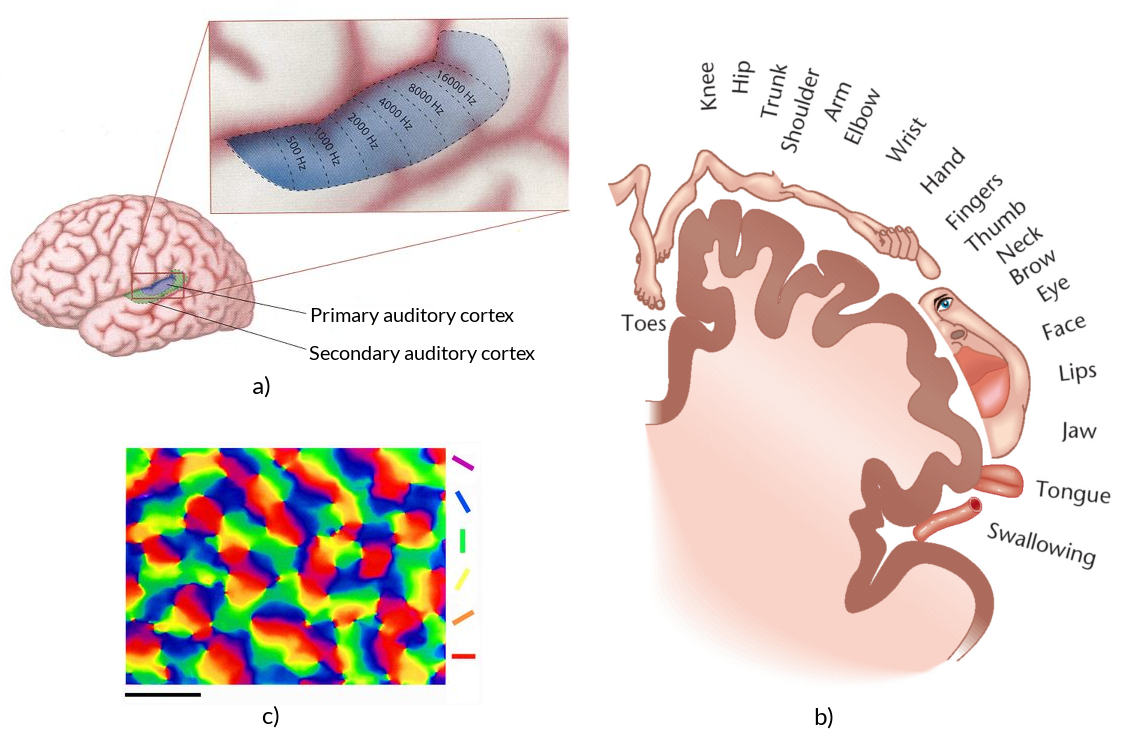
\epsfig{file=maps.png, height=10cm}
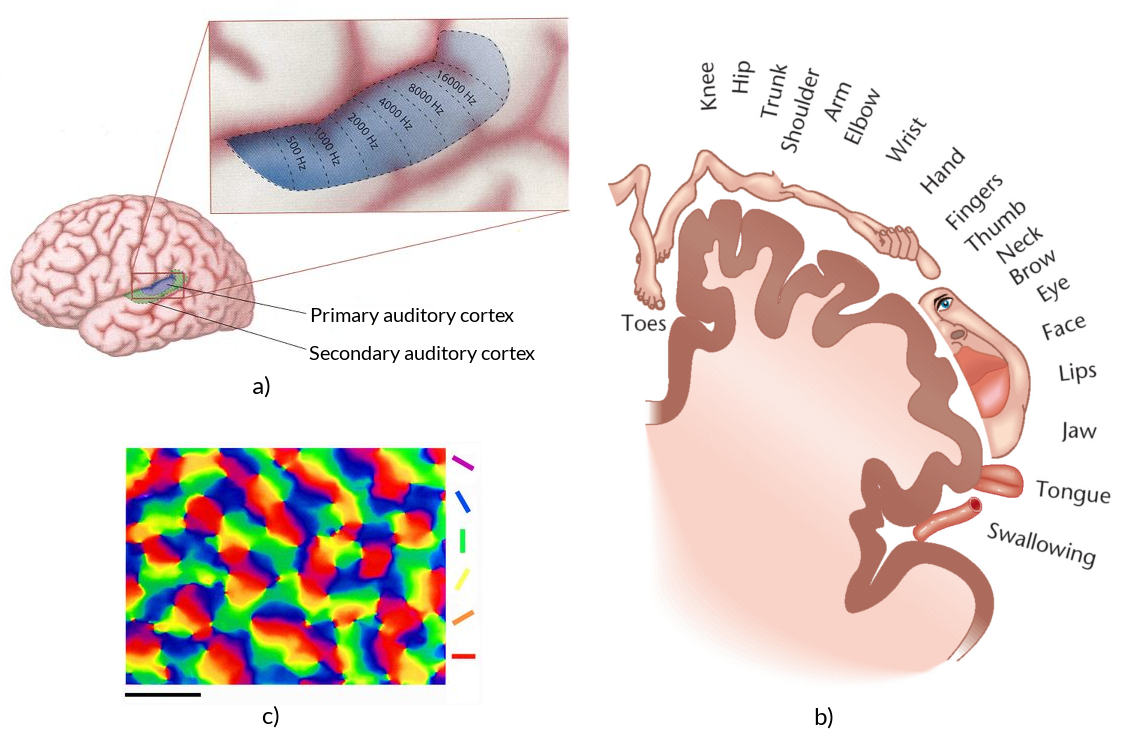
\includegraphics[scale=0.38]{maps.png}
\caption[Examples of topographic maps in the human brain]{Examples of
topographic maps in the human brain: cortical tonotopy (a), somatotopy (b) and 
orientation selectivity map (c). Images retrieved from: 
\url{
http://www.cns.nyu.edu/~david/courses/perception/lecturenotes/localization/loc 
alization-slides/Slide5.jpg}, \url{
http://images.scholarpedia.org/w/images/9/95/Visual_map_Swindale_Monkey_ori_doma
ins_Blasdel_1986.jpg}
and \url{http://spinacare.files.wordpress.com/2007/02/homunculus.jpg}}
\label{lab:tonotopy}
\end{figure}

The first years of an infant's brain development are characterised by stunning 
changes. By the age of three the brain has reached 80 percent of its adult 
volume \citep{SCI:Gil2007d, Nowakowski} and it has up to twice as 
many synapses as it will have in adulthood \citep{Krieg63}. Over time, in a 
process called \emph{synaptic pruning} redundant synapses are gradually 
discarded. The change in brain function and structure is known as \emph{brain 
plasticity} and is influenced by genetic and environmental factors. Greenough 
and Black \citep{GreenoughBlackWallace87} proposed a theory of two different 
types of brain plasticity: \emph{experience-expectant} (specific sensory 
experiences and input are needed at specific times for neural development and 
maturation) and \emph{experience-dependent} (interaction with the environment 
to develop skills for later use). The experience-dependent brain plasticity 
complies with the Vygotsky's theory on social development. Because genetic 
instructions are not sufficient to 
specify neural connections with sufficient precision, additional brain 
principles contribute to neural plasticity \citep{singer86}. One of these 
principles is \emph{self-organisation} which allows to optimise genetically 
determined blue prints of connectivity by shaping the structural and functional 
role of brain areas according to the sensory input. 
\newline
\phantom{x}\hspace{3ex} Here, we focus on the way sensory information is 
organised in the brain and analyse the influence of self-organisation. Sensory 
input to the human brain is often organised in the topographic structure. This 
means that adjacent brain regions process sensory inputs with similar features. 
Such regions are known as \emph{sensory maps}. Sensory maps in the human brain 
contain neurons specialised in encoding specific modalities of sensory input. 
The plasticity in these areas is driven by the gradual formation of internal 
representations across the lifespan \citep{helgeritter1990, ph2013development}. 
Tonotopic organization is a spatial arrangement in the auditory cortex where 
similar frequencies are processed by neighbouring brain regions. Orientation 
maps recorded in the visual cortex contain pinwheel formations where neurons 
exhibiting highest activities for certain orientations in the visual input are 
spatially grouped together. Finally, there are somatotopic maps such as 
the cortical homunculus that approximate cortical areas representing different 
body parts. All three maps are shown in Figure \ref{lab:tonotopy}. Neurons in 
that region show interesting \emph{self-organising} properties - if a part of 
the 
body is amputated, the neural correlate of that part will be ``overtaken'' by 
the neighbouring tissue increasing the sensation of the body part represented 
through that tissue. Merzenich \citep{merzenich:amputation} showed the 
reorganisation of cortical maps 
in monkeys before and after the amputation of fingers. This type of functional 
plasticity is known as cortical re-mapping.
The self-organising property also becomes evident in sensory maps throughout 
brain development. For example, Farah \citep{Farah98} argues that 
self-organization in somatosensory maps takes place in the womb while the pose 
of the foetus imposes mutual touching of the face and the hands, as well as the 
feet and the genitals. She proposes that this might be the reason why these 
body parts, although not close to each other physically, are represented close 
to each other in the brain. 

\subsection{Challenges in Modelling of Brain Development}
Unraveling neural mechanisms in a developing brain of a person acting in the 
environment is a very complex task due to several reasons. First, one would 
need to record brain activity over a sustained period of time where development 
occurs. Most current brain imaging techniques require a controlled setting that 
is hard to introduce as a part of everyday routine.
To record from brains of infants and young children, they should continuously 
participate in such experiments. Apart from dedicated involvement, there is a 
danger that in such a setting they might not behave spontaneously as they would 
when exposed to their usual environment. Second, it needs to be defined what 
level of brain activity should be recorded (i.e. smaller populations of neurons 
vs. brain areas), and how to relate anatomical and functional changes of a 
developing brain within the social and cultural context. Developmental robotics 
in combination with biologically realistic brain models might help set the 
ground for this investigation. Robots equipped with artificial neural networks 
that capture ongoing development provide a controlled environment 
to analyse and steer learning mechanisms infants might employ when interacting 
with humans. 
%In this way, investigation of a developing brain might be more feasible based 
%on cues obtained via experiments with robots. 

In this thesis, the knowledge about the developing brain from studies 
with animals, as well as lesion studies in human brains, has been utilised to 
develop a computational model based on artificial neural networks.
Two properties of the developing brain, self-organisation and topology 
preservation, have been phenomenologically captured using the model.
Implementation of the model on a robotic platform accounts for a realistic 
sensory experience, that might simulate those of a small child throughout the 
early stages of development. 

\chapter{Materials and Methods}
\label{chap:methods}
%\pagenumbering{arabic}

In this chapter we describe the model implemented on a robot for learning of sensorimotor competences at early stages of development in children. 
We start by explaining the development of hand-eye coordination in \ref{sec:hecoord}, an important motor skill that develops early in infancy. We proceed by explaining the body babbling (mentioned in section \ref{sec:devsoccog}) algorithm  implemented on a robot. Then, we introduce the biologically inspired model based on self-organising maps in section \ref{sec:themodel}. We explain the biological motivation, the model architecture and implementation details. Finally, in section \ref{sec:modeltrain} we explain how data acquired through random body babbling is used to tune the model.

\section{Hand-Eye Coordination}
\label{sec:hecoord}

Control of limbs is one of the first motor skills which humans learn.
Hand-eye coordination is acquired early in infancy where visual input is used to control, guide and direct hand movements. 
Vision in infants develops gradually and is largely dependent upon the bodily experience \citep{pmid9455172}. For example, infants at the age of 3 months exhibit saccadic movements only in the retinocentric reference. At the age of 3 or 4 months ``hand regard'' behaviour is observed when they are able to gaze at their own hands moving in front of their faces. At the age of 7 months they perform saccadic movements in the body-centered reference frame.
Visual guidance is thus essential for the development of gross and fine motor skills that are used in everyday interactions with the environment.
Ability to coordinate finger and arm movements, grasping, reaching, and the ability use hands to manipulate objects is known as \emph{dexterity}. 
Dexterity in artificial agents such as robots remains a difficult challenge due 
to several reasons. 
For example, depending on the number of degrees of freedom, there could 
be infinite many arm configurations that result in the same hand position. 
It is the task of a roboticist to determine what arm configurations are feasible and how to deal with the curse of dimensionality due to many degrees of freedom of the robot's arm. Another example is the problem of depth perception when using a single camera for visual input. Without depth information the robot is not able to point because of a similar reason - there are many different arm configuration resulting in the same perceived marker position (Figure \ref{lab:handpositions}). To address these problems we analyse learning mechanisms infants employ to acquire similar skills.
In the early stages of development infants gradually learn to acquire  sensorimotor coordination.
They learn configurations of arm postures through a set of self-exploration activities such as body babbling. 

\begin{figure}[h]
\centering
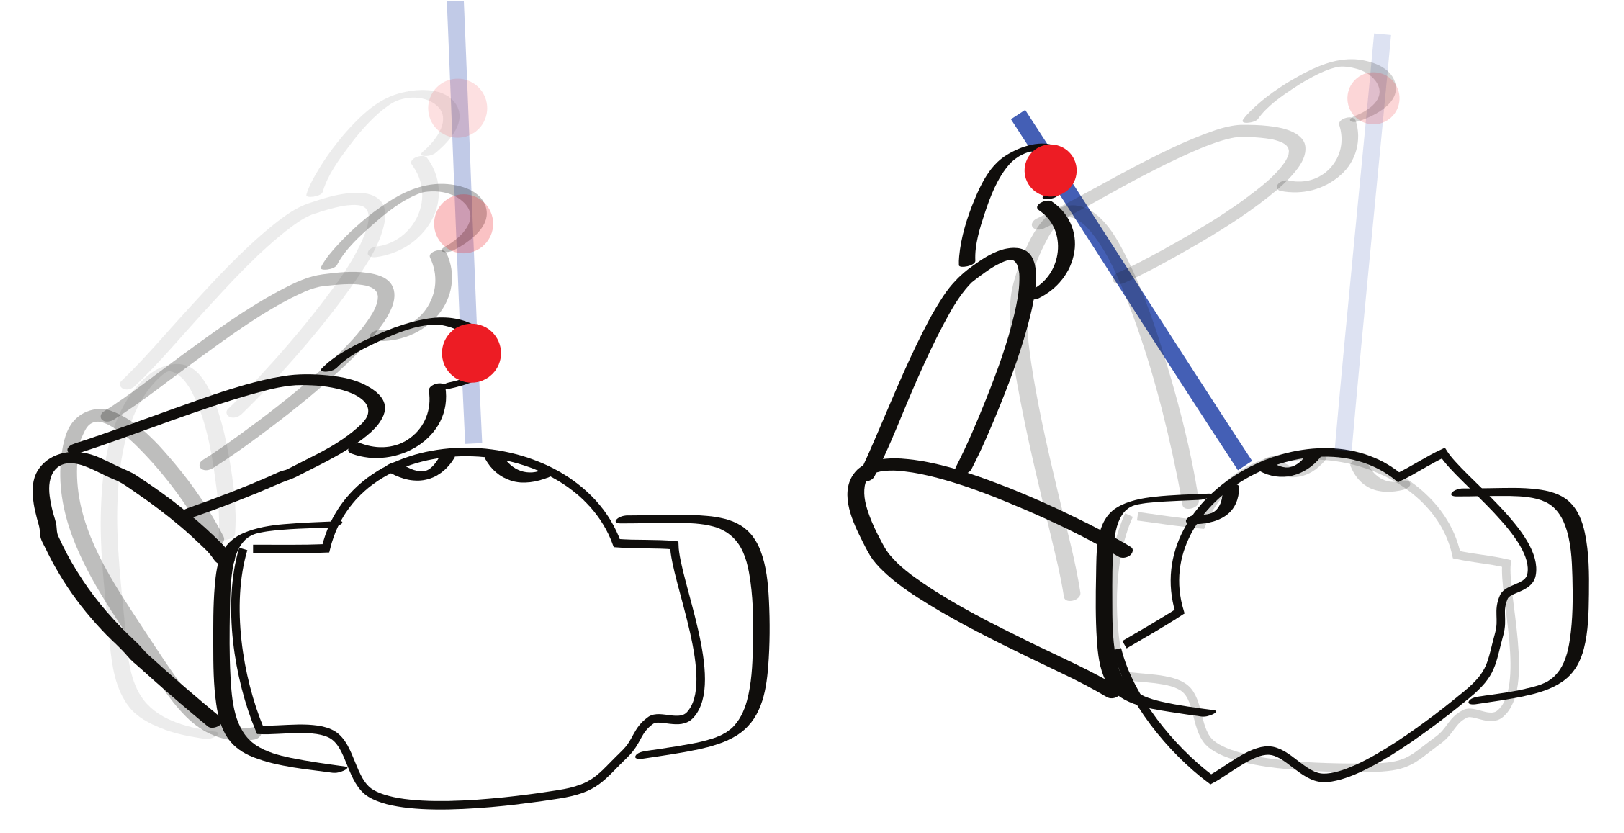
\epsfig{file=multiple_config.png, height=4cm}
\caption{Multiple arm configurations result in the same perceived marker position}
\label{lab:handpositions}
\end{figure}


\subsection{Random Motor Babbling}
\label{sec:babbling}

Body babbling employed by infants is motor experience for mapping movements to the resulting body configurations \citep{Meltzoff97}. 
To avoid exploring the whole set of possible arm configurations, infants 
constantly try to reach objects surrounding them even if that reaching results 
in failed actions. As explained in the chapter \ref{sec:devsoccog}, it is 
assumed that pointing emerges from such failed reaching actions which are 
interpreted as the infant's request for an object. 
%The idea that infants do not employ purely random babbling gestures underlies the theory of goal babbling.
Body babbling is fundamental in learning of limb postures and correlations between motor actions and resulting sensory input. In developmental robotics, body babbling can be used for the acquisition of basic motor competences such as hand-eye coordination \citep{Lungarella2003} that eventually lead to the development of more complex behaviours such as sharing of the attention through pointing \citep{Hafner2011}. 
There are several limitations to the random body babbling algorithm, such as inability to switch between exploration of new postures and exploitation of existing ones based on robot's learning interest. Goal directed behaviours have been proposed in \citep{olsson2006} and \citep{baranes2013}, showing that it is possible to gradually integrate information about the robot's sensory system in a developmental paradigm. However, the scope of this thesis does not deal with such advanced exploration behaviours.

\begin{figure}[t]
\centering
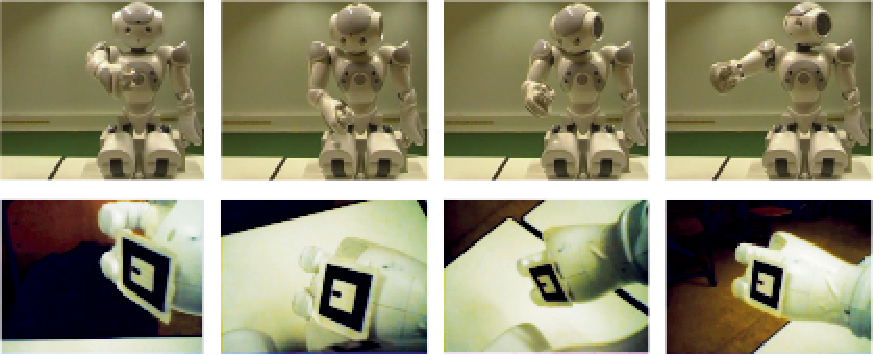
\epsfig{file=sequence.pdf, height=5cm}
\caption{A sample sequence of random motor movements during motor babbling in a robot}
\label{lab:babbling}
\end{figure}


Several robotics studies have been inspired by the infants' behaviour of body babbling.
Exploration behaviours have been implemented in artificial agents for gathering 
evidence to form internal models of their bodily characteristics 
\citep{SchillaciHLG13, Saegusa2009}.
Schillaci et al. propose a way for combining knowledge through exploration and 
knowledge from others \citep{SchillaciHLG13}, and Demiris et al. use mirror 
neuron inspired internal models \citep{Demiris2005}.
An exploration mechanism driven by the active 
self-generation of high-level goals has been proposed by Baranes 
\citep{baranes2013}. Such a mechanism allows active learning of inverse models 
in high-dimensional redundant robots. 

In this thesis acquisition of coordination skills through random 
motor babbling has been implemented on a humanoid robot Nao from Aldebaran. 
Physical dimensions of the Nao resemble those of a child standing at a height of 
ca. 57 cm and simulating the real visual input perceived by a young human 
subject. A sample babbling sequence is shown in Figure \ref{lab:babbling} where 
the first row shows random hand movements, and the second row the corresponding 
frames captured by the camera. The implementation of the babbling procedure was 
adapted from \citep{SchillaciH11}. The robot has been provided with a simple 
behaviour based on sensorimotor coordination which allowed it to look at its own 
random arm movements. In particular, the behaviour consisted of the following 
steps: a motor command, that is, a desired angle position, is sent to each joint 
of the arm (only one arm is babbling); when the hand of the robot, represented 
for simplicity by a marker\footnote{We used the ARToolkit library for marker 
detection (http://www.hitl.
washington.
edu/artoolkit).}, is detected, the joints of the neck are rotated in order to center the marker in the perceived visual input. 
The bottom camera placed in the robot's head has been used to capture the visual input at a varying speed between 9 and 30 frames per second.
During the babbling process, information related to the estimated position of the marker is stored and mapped with the current configuration of the arm joints in a knowledge base. 
The position of the marker is characterised by a horizontal, vertical and depth dimension. The depth dimension is computed based on the dimensions of a marker provided through a configuration file to the ARToolkit library.
Four arm joints have been used: shoulder pitch, shoulder roll, elbow yaw and elbow roll. 
%Together, the marker position and positions of joints form a 7D data point. 

By implementing the random motor babbling algorithm on a robot we make several assumptions regarding the development of sensorimotor skills. First, we assumed that the ``hand regard'' behaviour is already learned since the robot is able to gaze at its moving hand. By equipping the robot with a system for marker detection, we shortcuted a part of the developmental trajectory which is known to exist in infants. 
In \citep{Metta2000} this stage of the development has also been learned, in addition to acquisition of numerous other sensorimotor skills.
Second, there exists evidence for goal babbling \citep{rolfs2012}, stating that infants already few days after birth try to reach goals, although they constantly fail. Using a random walk strategy we excluded the role of goal-directed behaviours. We made these assumptions because this thesis does not concern itself with the extent to which sensorimotor skills are innate or learned.

\section{The SOM-based Model}
\label{sec:themodel}

We aim to develop a model for coding sensorimotor experience inspired by computational properties of sensory maps in the human brain (section \ref{ssec:braindev}). In particular, we phenomenologically simulate experience-dependent plasticity in the model based on the robot's interaction with the environment. In the human brain, sensory maps contain neurons specialised in processing of information coming from specific sensory modalities. Our model is motivated by two characteristics of sensory maps: topological structure and the self-organising property. 

\subsection{Simulating Sensory Maps}
\label{sec:simsensmaps}

Sensory maps can be simulated using artificial neural networks (ANNs), which are 
computational algorithms inspired by the brain organisation and structure. 
Expressed using mathematical vocabulary, an ANN is a graph whose nodes are 
neurons organised in a layered architecture and connecting edges among them are 
neural weights. Weights are computed using various learning rules such as 
backpropagation algorithm or gradient descent. Resulting weights accomplish 
mapping of the input values to the desired outputs by approximating an initially 
unknown function which describes that relation.
In the mathematical theory of neural networks, they are called universal function approximators (for mathematically rigorous description see \citep{Kurt1991251}).
ANNs do not capture the exhaustive level of information processing detail as observed in real biological systems. They rather attempt to reproduce experimental data by taking the same stimulus as input, or are used to computationally reproduce phenomena observed in neural systems. 

Based on insights into the way the brain represents and manipulates sensory information presented in section \ref{sec:neurosci}, we decided to a use a particular class of ANNs known as \emph{self-organising maps} (SOMs) or Kohonen networks \citep{Kohonen}. 
SOMs have been widely utilised in modelling of formations of different sensory modalities such as those in the auditory cortex \citep{MartinezRitterSchulten1988}, somatotopic maps \citep{Obermayer:1990} and orientation maps in the striate cortex \citep{malsburg73}.
Also, SOMs are well suited for learning hand eye-coordination without a priori model of arm kinematics in the simulated \citep{Marggie94} as well as the physical \citep{Martinetz} robotic arm. 
One of the reasons for using a biologically-inspired model is to gain better 
understanding of the biological system through computational modelling. We use a 
brain-inspired Hebbian learning paradigm to associate maps to simulate 
interaction between brain areas based on the interaction of the agent with the 
external world.
 
In \citep{Kohonen} an explanation is provided that states the relation between formalisms behind SOMs and physical or neural systems. In another words, it is possible to express biological processes or mechanisms in terms of mathematical formulas or algorithms. Two relations between SOMs and neural systems are identified which can be studied independently: formation of an activity cluster around the neuron with the maximal activity (1) and the adaptive change in the input weights of those neurons where activity was confined (2). The phase (1) is supported by the anatomical and physiological evidence for lateral interaction between neural cells: short-range excitation and long-range inhibition (Figure \ref{fig:interact} (a)). A schematic representation of a network  which may implement such a function is shown in Figure \ref{fig:interact} (b). The phase (2) is related to limited synaptic resources such as 
neurotransmitters and energy, and the change of synaptic efficacy depending on the type and location of the synapse.



\begin{figure}[t]
\centering
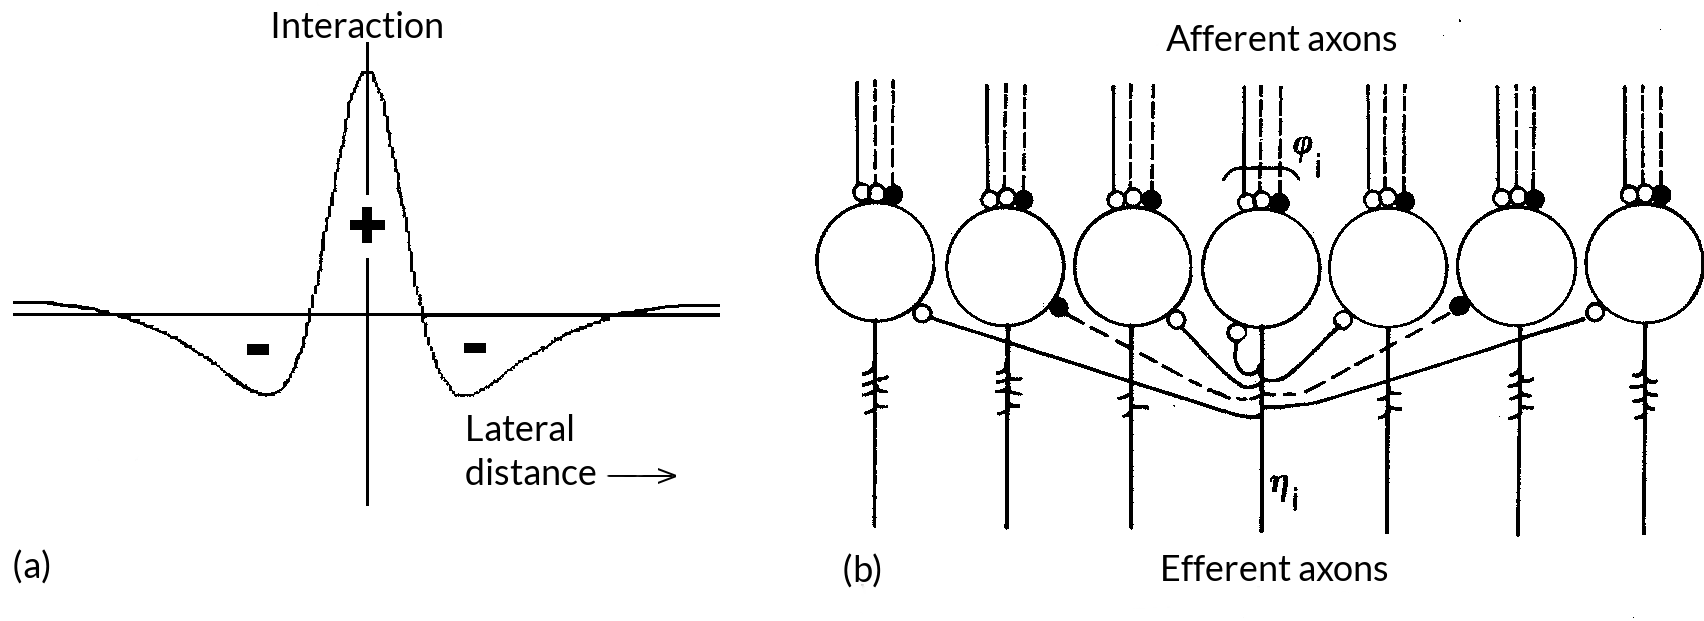
\includegraphics[scale=0.25]{soms_bio_hor.png}
%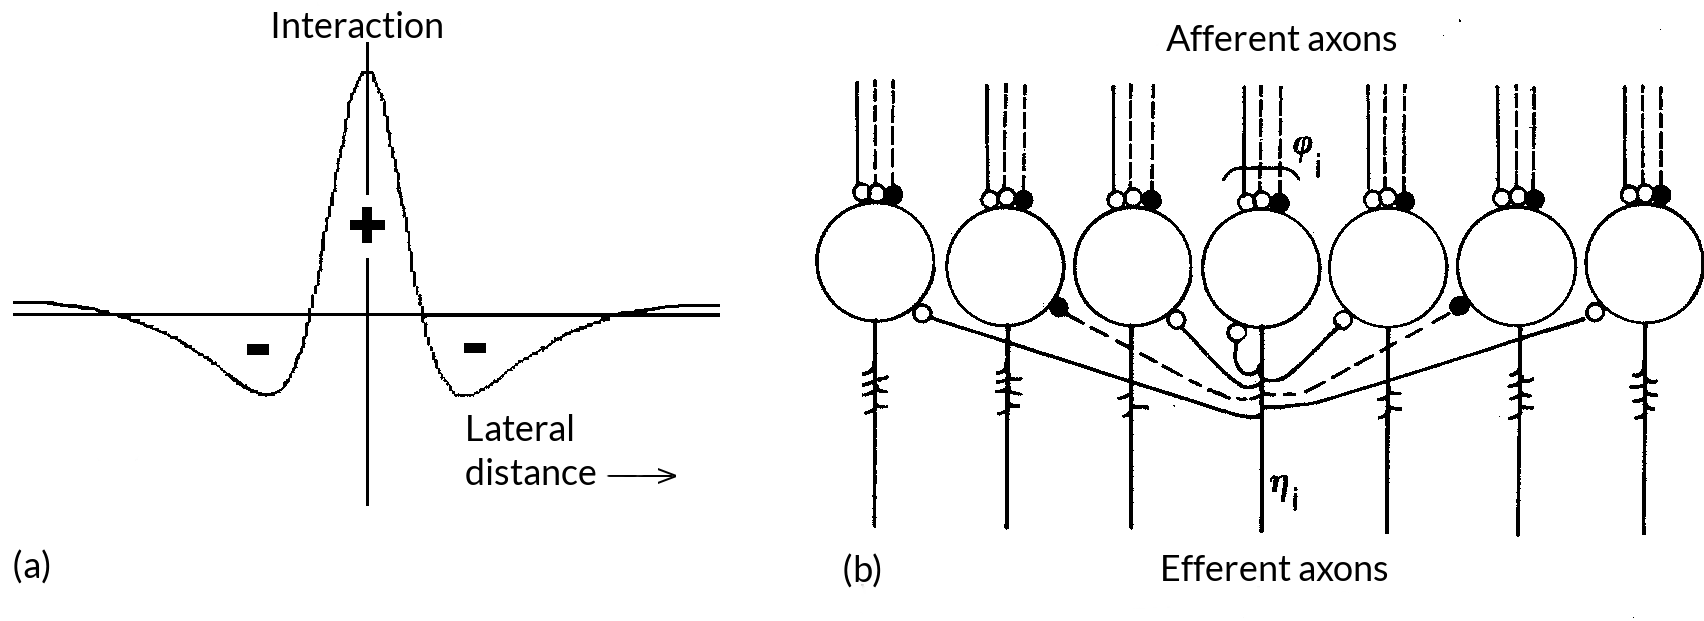
\epsfig{file=soms_bio_hor.png, height=5.5cm}
\caption[Lateral connectivity around the winning neuron in a SOM]{Profile of the function describing the interaction of the winning neuron and neighbouring neurons (a) and schematic representation of lateral connectivity which may implement that function (b) (Figure adapted from \citep{Kohonen})}
\label{fig:interact}
\end{figure}



\subsection{Formalisms behind SOMs}
\label{sec:sommath}


A SOM is constructed as a grid of neurons, where each neuron is represented as 
an $n$-dimensional weight vector $\mathbf{w_i}$. Neigbouring neurons are 
connected in a topological structure.
The number of dimensions of a weight vector corresponds to the dimensionality of input data. Each neuron approximates a certain region of data points in the input space yielding less units needed to represent the input. For this reason, one often refers to SOMs in terms of dimensionality reduction algorithm which is not to be confused with algorithms such as PCA, SFA or ICA which aim to find the low-dimensional representation of the input.

Weights in the network are initially set to random values and then adjusted iteratively by presenting the input vector $\mathbf{x_p}$ which is randomly chosen from the input data. In each iteration, the winning neuron $i$ is selected as a neuron whose weights are closest to the input vector in terms of the Euclidean distance:
\begin{equation}
\underset{i}{\arg\min} || \mathbf{x_p}-\mathbf{w_i} ||
\end{equation}
After selecting a winning neuron, the weights of all other neurons, here denoted as $j$, are adjusted:
\begin{equation}
\mathbf{\Delta w_{j}} = \eta(t) h(i, j) (\mathbf{w_{j}}-\mathbf{x_p})
\end{equation}

The $\eta(t)$ parameter is a learning rate which defines the rate at which the weights are changed.
The function $h(i, j)$ is a Gaussian neighborhood function defined over the grid of neurons as:
\begin{equation}
%h(i, j)=e^{(\frac{\mathbf{w_i^2}-\mathbf{w_j^2}}{2\pi\sigma(t)^2})}
h(i, j)=e^{-\left(\frac{\mathbf{w_i^2}-\mathbf{w_j^2}}{2\pi\sigma(t)^2}\right)}
\end{equation}

The profile of the Gaussian neighborhood function is inspired by the lateral connectivity profile as shown in Figure \ref{fig:interact} (a). The function is centered around the winning neuron $i$ and its values are computed for all neurons $j$ in the grid.
 The spread of the function determines the extent to which neighbouring weights of a winning neuron are going to be affected in the current iteration. The topology of the network is preserved by pulling together neurons closest to the winning node.  
The learning rate $\eta$ and the spread of the Gaussian function $\sigma$ are held constant for the first half of iterations, and afterwards are annealed exponentially. This underlies the assumption that the initial configuration of neurons in the network poorly covers the space, and only upon iterative presentations of input data starts converging to the optimal state.

The activation function of a neuron, $A(\mathbf{x})$ is computed over the Euclidian distance ($\textbf{x}$) between the neural weights and the input vector:
\begin{equation}
A(\mathbf{x}) = \frac{1}{1+\tanh(\mathbf{x})}
\end{equation}

It is a common practice in cognitive modelling to connect multiple SOMs using the associative links \citep{Morse2010}, \citep{Westerman02modellingthe} and \citep{COGS:COGS716}. The Hebbian learning paradigm describes an associative connection between activities of two connected neurons. If a postsynaptic neuron $j$ is always activated after the presynaptic neuron $i$, the connection between these two neurons is strengthened using the following rule:
\begin{equation}
\Delta w_{ij} = \eta_h A(\mathbf{x_i}) A(\mathbf{x_j})
\end{equation}

Vectors $\mathbf{x_i}$ and $\mathbf{x_j}$ are distances between winning neurons and the corresponding inputs in two different maps.
Initially, all weights between two SOMs are set to zero allowing for an activity-dependent role of structural growth in neural networks.


\subsection{Model Architecture}

The inspiration for the model architecture comes from the Epigenetic Robotic 
Architecture (EPA) which was proposed as a framework for guiding modelling 
efforts \citep{Morse2010}. The basic ERA unit consists of SOMs connected via 
Hebbian weights to a central SOM acting as a ``hub''. Depending on the use case, 
different ERA units can be associated to different brain regions depending on 
the type of information they represent or the type of processing. For example, 
maps are used to represent different physical features such as the color space, 
the body posture and the word space. The architecture is implemented on a 
humanoid robot iCub and is capable of reproducing a wide range of psychological 
phenomena with results comparable to those obtained in experiments with humans. 
It is not tailored to specific domains or tasks, making it suitable for 
extensions and novel applications. In addition, it displays an ongoing 
developmental trajectory providing a ground to analyse learning behaviours of 
agents 
interacting with the environment.

Based on guiding lines provided by the ERA, we decide to associate two 2D SOMs.
Each SOM represents a different part of the left arm posture. Neurons in each SOM are ordered in a grid consisting of rows and columns, such that each neuron is identified by a 2D index. This is schematically depicted in Figure \ref{lab:model} where the ``blue'' SOM is used to represent the elbow and shoulder positions, and the ``red'' SOM the hand positions. Every neuron in the ``blue'' SOM is identified through a 3D weight vector ($x, y, z$), and every neuron in the ``red'' SOM through a 4D weight vector ($\sigma_p, \sigma_r, \epsilon_y, \epsilon_r$). The weights of neurons in the first SOM are meant to represent vertical, horizontal and depth dimensions, while weights in the second SOM stand for shoulder pitch, shoulder roll, elbow yaw and elbow roll. Those weight are later used when issuing a motor command to the robotic arm.
Arrows in the figure depict Hebbian weights, such that thicker arrows represent stronger synaptic connections. Different instances of a model are named according to the number of neurons in each row and each column in a single SOM (e.g. \ssom model or \bsom model). 

\begin{figure}[t]
\centering
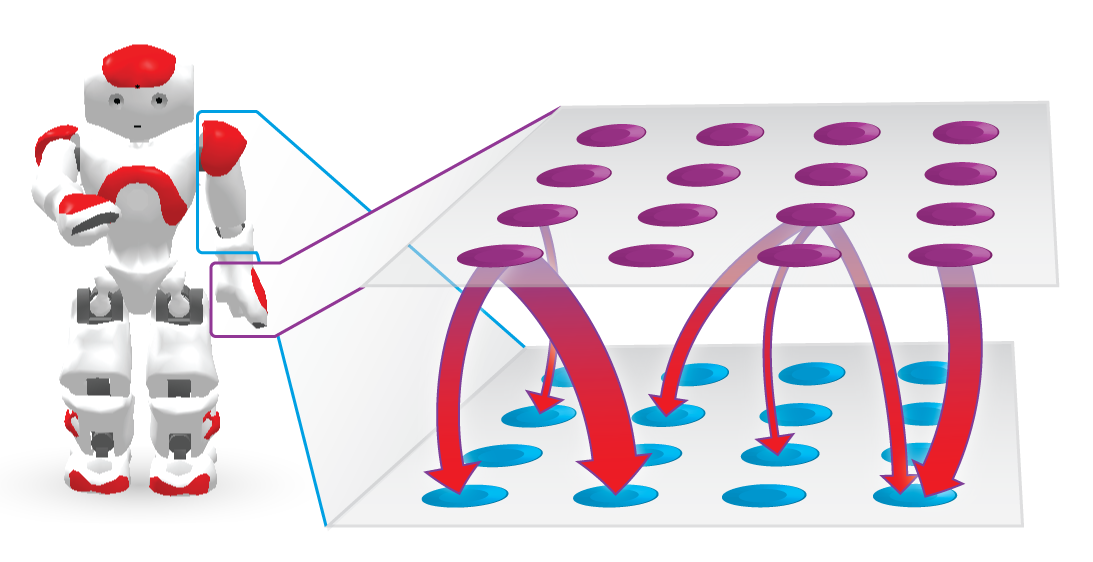
\epsfig{file=model.png, height=6cm}
\caption{Scheme of the model architecture for learning hand-eye coordination with SOMs and connecting weights}
\label{lab:model}
\end{figure}

\section{Training Data}
\label{sec:modeltrain}

The weights of neurons were adjusted using the data obtained in the babbling experiment. 
From the knowledge base constructed in the babbling experiment, two training sets were created. One training set comprised of the 3D hand coordinates and the other of 4D joint coordinates.



\chapter{Experiments}
\label{chap:experiments}

\section{Data Acquisition through Random Motor Babbling}
\label{sec:exp-mb}
The goal of the motor babbling experiment is to simulate the acquisition of hand-eye coordination as it occurs in infants. 
As a result, robot's limb postures achieved in the experiment, characterised through absoulte positions, were stored in a knowledge base.
By equipping the robot with the SOM-based model and using data in the knowledge base we hope to simulate a part of infants' developmental trajectory in an artificial agent. 

The babbling procedure with a random walk strategy has been adapted from 
\citep{SchillaciH11}. Random steps which involve increasing, holding or 
decreasing the joint by angle-step are sampled from a uniform distribution. 
Random steps are iteratively added to the current configuration and the ranges 
of joint configurations in degrees are: for shoulder pitch from -120 to 120, for 
shoulder roll -95 to 0, for elbow roll from 0 to 90 and elbow yaw from -120 to 
120. Only a maximum step of 10 degrees is allowed for each joint. If the 
randomly determined arm position is impossible to reach due to physical 
constraints of the robot's arm, a new position is chosen until the generated 
position is possible. The experiment consisted of a robot randomly babbling with 
its left hand while looking at its own arm movements. Such behaviour consisted 
in the robot moving its arm in a random fashion and generating head movements 
according to the visual perception of its own hand which was tagged with a 
marker. At each time step, which was determined by the capturing rate of the 
camera, positions of the arm were stored in a knowledge base. While the robot 
moves its arm, it estimates the position of its hand by analysing the visual 
input and moves. It moves joints of its neck in order to keep the hand in the 
center of the image. The 3D position of a marker is computed relative to the 
robot torso.

Two babbling experiments were conducted to collect the data. The first experiment lasted for approximately 40 minutes and it yielded 74,143 data points. These data points were used to train the SOM-based models that were implemented on a robot. The second babbling experiment lasted approximately 30 minutes during which 57,778 data samples were collected. This data set was used to check the quality of the model prior to implementation on the robot. The motivation for the quality assessment arose after we tried to use babbling data obtained in a computer simulation for the training of the model. In that case, instead of gathering data via the babbling experiment we used Webots, a software for simulating robots on a computer, to simulate babbling experiment and collect data. When the model trained on this data was implemented on a robot and used in the experiment the pointing was very imprecise. Moreover, the robot's movements appeared almost random disrupting the natural flow of human-robot interaction. The 
reason for this poor performance might have been the lack of noise and ideal conditions imposed by the simulation environment which did not realistically depict the experimental setting. Motivated by the difference between the simulated and the real environment, we decided to perform an additional babbling experiment to check the model performance prior to implementing the model in a robot. 


\section{Model Training}
\label{sec:exp-modtrain}

\subsection{Adjustment of Weights}
The training of the model consisted of two phases. In the first phase, only the 
local neural weights in each SOM were adjusted. In total, there were 20,000 
iterations in which an input vector was randomly chosen from a babbling 
knowledge base gathered in the first babbling experiment. The input vector was 
a 7D vector, which was divided into the 3D hand vector and the 4D joint vector. 
The hand vector was presented to the first SOM and the 4D joint vector to the 
second SOM. Winning neurons in both SOMs were detected as the ones with the 
lowest Euclidean distance to the input vector. Weights of winning neurons and 
neurons surrounding them were adjusted according to the formulas explained in 
the section \ref{sec:sommath}.
In the second phase, the winning neurons in both SOMs were associated using the Hebbian learning rule which defined the connection strength based on their level of activation.

\subsection{Training Parameters}
The learning rate $\eta$ was set to 0.9 and the spread of the Gaussian neighbourhood function $\sigma$ was 0.7. Both hyperparameters were kept constant for the first half of iterations, and afterwards annealed exponentially. The scaling factor used to associate neurons between the two SOMs, $\eta_h$ was set to a constant value 0.01 ensuring the positive weight growth.\\

\subsection{Model Configurations}
We trained three different instances of a model: the $5\times 5$ model consisted of two 2D SOMs with each SOM having 25 neurons, the $10\times 10$ model consisted of two 2D SOMs with each SOM having 100 neurons and the $15\times 15$ model with 225 neurons in each SOM. In addition, we investigated the influence of the training data on all three models and present the results in the following section. In the same section we tested all three models using the second babbling data set to measure pointing accuracy.
The $5\times 5$ and the $15\times 15$ model were implemented on the humanoid robot and used in an experiment with a human. The SOM covering the hand space from the $5\times 5$ model is shown in Figure \ref{lab:5x5} and the same SOM from the $15\times 15$ model is shown in Figure \ref{lab:15x15}. 
The motivation for investigating models of different sizes comes from the assumption that bigger networks might evolve from the smaller ones. In this way, the progression of skill development is followed by the increased number of neurons specialized in coding od sensorimotor experience. All models were trained using the same parameters.

\begin{figure}[t]
\centering
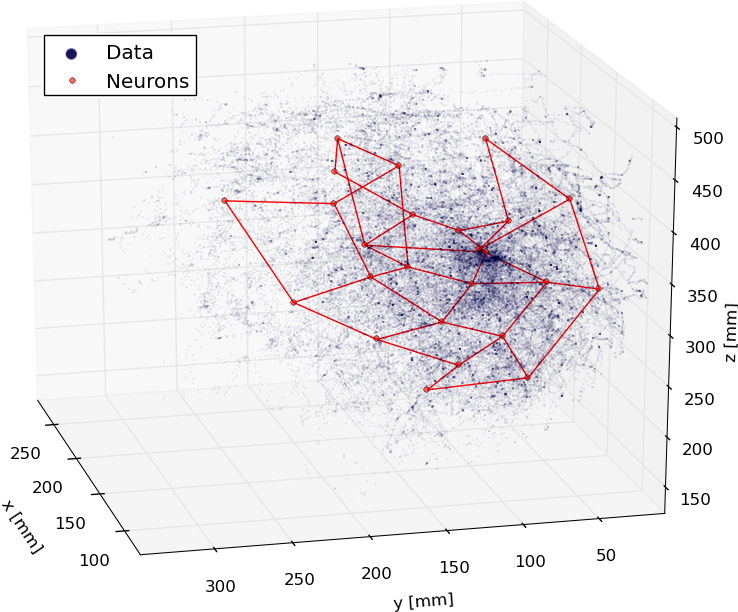
\includegraphics[scale=0.55]{SOM_5x5.png}
%\epsfig{file=SOM_5x5_zoom.png}

\caption{The SOM with 25 neurons approximating the left hand trajectory samples in the \ssom model}
\label{lab:5x5}
\end{figure}

\begin{figure}[t]
\centering
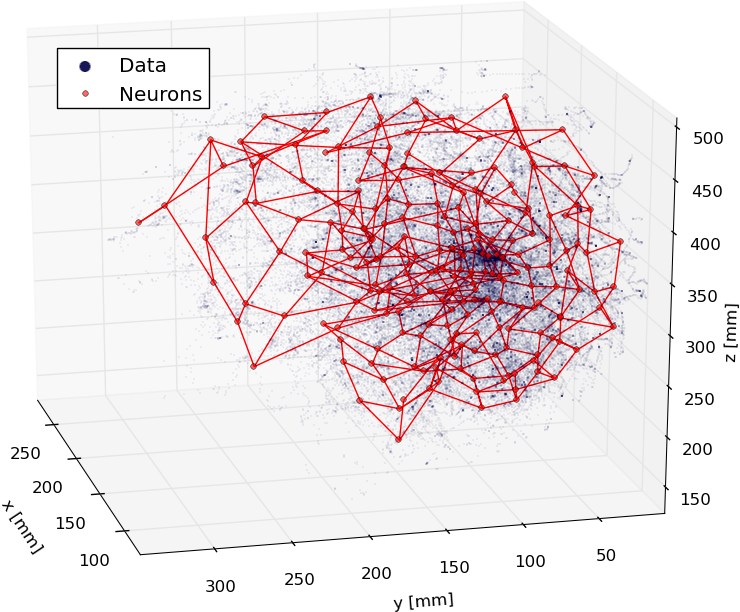
\includegraphics[scale=0.55]{SOM_15x15.png}
\caption{The SOM with 225 neurons approximating the left hand trajectory samples in the \bsom model}
\label{lab:15x15}
\end{figure}

% \begin{figure}[h]
% \centering
% \epsfig{file=hebb.png, height=6cm}
% \caption{Hebbian weights}
% \label{lab:5x5}
% \end{figure}


\section{Preliminary Results}
The goal of preliminary computational experiments is to investigate the quality of models prior to the implementation on a robot. This is a sanity check that ensures there are no errors or bugs in the program that might be hard to detect once the model is implemented on the robot.
First, we trained the three models on the the data gathered in the first babbling experiment. Second, we altered the training procedure in two ways: either by picking only the first $p$ fraction of the points from the babbling session, simulating a shorter babbling phase, or by picking every $n$th data point, thus simulating a babbling process that was slightly ``sped-up''. All models were tested only using the data points from the second babbling experiment.

The testing procedure comprised of presentation of a 3D hand vector to the first SOM, activating a winning node and computing the Euclidean distance between them. In table \ref{lab:table_trainf} we present errors for all models that were trained on different amounts of data, but where training data points were picked uniformly such that each $n$th point was chosen.

\renewcommand{\arraystretch}{1.5}
\begin{table}[t]\footnotesize
\begin{center} 
 \caption{Errors for all three models and training sets using approximately first $p$ percent of training data}
 \label{lab:table_trainf}
 \begin{tabular}{|c|c|c|c|}
   \hline     
    p= & $1\%$ data & $10\%$ data & $100\%$ data\\ \hline
   $5\times 5$ & $46.00 \pm 37.75$ & $29.82 \pm 18.15$ & $29.11 \pm 14.99$ \\ \hline
   $10\times 10$ & $39.65 \pm 37.96$ & $21.44 \pm 17.22$ & $18.87 \pm 11.68$ \\ \hline
   $15\times 15$ & $39.45 \pm 38.23$  & $17.82 \pm 15.78$ & $14.18\pm 8.30$ \\  
   \hline
 \end{tabular}
\end{center}
\end{table}

We see that the increase in number of neurons is followed by the lower error and that  models trained on more data perform better. From computational point of view this result is expected as more neurons provide higher resolution of the input space. However
In table \ref{lab:table_trainu}, we show the three models trained on different amounts of data where training points were used only from the beginning of the babbling set.

\renewcommand{\arraystretch}{1.5}
\begin{table}[h]\footnotesize
\begin{center} 
 \caption{Errors for all models and training sets using every $n$-th data point}
 \label{lab:table_trainu}
 \begin{tabular}{|c|c|c|c|}
   \hline     
    n= & $100$ ($1\%$ data) & $10$ ($10\%$ data)\\ \hline
   $5\times 5$ & $29.48 \pm 15.98$ & $28.92 \pm 14.45$  \\ \hline
   $10\times 10$ & $18.66 \pm 11.48$ & $18.43 \pm 10.29$ \\ \hline
   $15\times 15$ & $14.33 \pm 9.03$  & $13.90 \pm 7.95$\\  
   \hline
 \end{tabular}
\end{center}
\end{table}

As expected, if training points were chosen randomly from the whole babbling set compared only to the first $n$ points, the errors were much lower. 
In addition it is interesting to notice that models trained only on 1\% (cca. 700 data points) of the randomly chosen training data were performing just slightly worse (or approximately equal) than the models trained on the 100\% of the data. 

\section{Human-Robot Interaction}
\label{sec:exp-hri}

\begin{figure}[h]
\centering
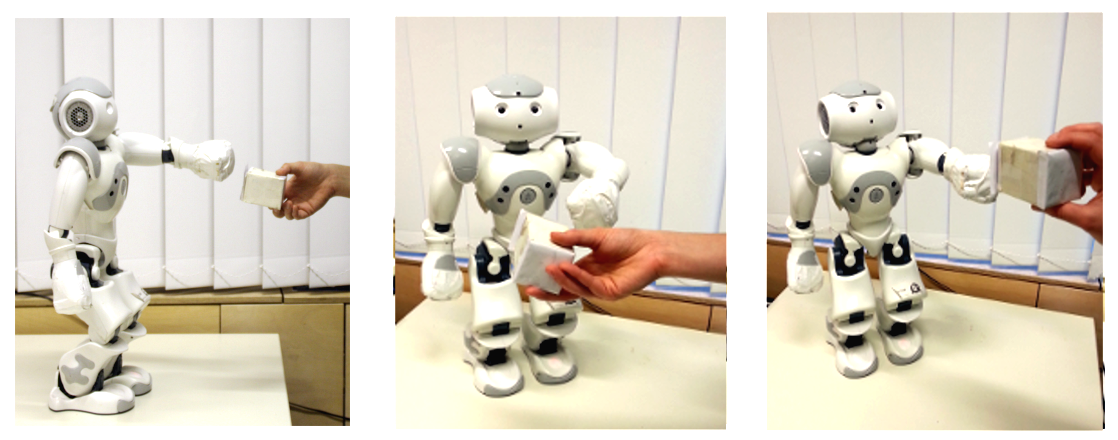
\epsfig{file=experiment_new.png, height=5cm}
\caption{Pointing sequence in a human-robot interaction}
\label{lab:experiment}
\end{figure}

Both the \bsom and \ssom models trained on data acquired in the babbling experiment were implemented on a robot. The robot equipped with models was standing in front of a human subject on a table as shown in Figure \ref{lab:experiment}. The experimenter held an object tagged with a marker and moved it randomly within the visual field of the robot. The movements were performed at a varying speed, trying not to exceed the speed of the robot's moving hand. The experimenter tried to cover the space within and beyond the reach of the robot's hand to explore the extend of possible arm configurations. While the object was moved in front of the robot, it followed the marker with its arm and gaze. For positions within the reach of its hand, the robot bended the arm to point to the object. For positions beyond the reach of its hand, the robot extended the arm in the direction of the object. This action was interpreted as pointing. The experiment took place for approximately 2.5 minutes and the arm position 
characterised through hand and joint coordinates was stored every 100 ms on a memory disk in the robot. As seen in the 
figure, the problem of various arm configurations resulting in the same hand positions was successfully resolved using the SOM-based model.

In the experiment with a human subject, the \bsom model was used to determine the left arm position at every time step a marker was detected. The procedure to determine the arm configuration was following. First, the robot detected 3D marker coordinates using the camera in its head. Marker coordinates were described as a 3D vector containing the horizontal, the vertical and the depth dimension ($\mathbf{w_m}$). 
The 3D vector was presented to the first SOM and a winning neuron $\mathbf{w_i}$ was selected such that: 
\begin{equation}
\underset{i}{\arg\min} \hspace{1mm} ||\mathbf{w_m}-\mathbf{w_i} ||
\end{equation}

Based on the strongest Hebbian connection from the winning neuron $i$ in the first SOM, a neuron $j$ in the second SOM was selected such that: 
\begin{equation}
\underset{j}{\arg\max} \hspace{1mm} w_{hebb}(i, j) 
\end{equation}

$w_{hebb}$ denotes Hebbian weights estimated in the training process.
Weights of a winning neuron ($\sigma_p, \sigma_r, \epsilon_y, \epsilon_r$) in the second SOM were used to issue the motor command to set arm joints. The first two dimensions of a weight vector ($\sigma_p, \sigma_r$) were used to set the shoulder pitch and shoulder roll, and the two second dimensions ($\epsilon_y, \epsilon_r$) to set the elbow yaw and elbow row. Concurrently to the activation of a winning neuron in the second SOM of a \bsom model, the winning neuron in the second SOM of a \ssom model was detected. The procedure was the same for both models, but the weights of a winning neuron in the \ssom model were not used to steer arm kinematics. They were stored and used for comparison between the object position, and the winning weights of the \bsom model.



\chapter{Results and Discussion}
\label{chap:discussion}

% \section{Results}
% \label{sec:results}

Due to the interdisciplinary nature of this work the results can be analysed from several different perspectives. We start with a quantitative analysis of the pointing precision in the experiment, defined by the Euclidean distance metric. The performance of the two models implemented in the robot is compared in terms of the lowest pointing errors. Then, we focus on the implications of the model and its results for neuroscience, developmental psychology and cognitive robotics. Finally, we discuss possible extensions and improvements of the model and the experimental setting by proposing future research directions.



\section{Quantitative Analysis}

In this section we compare the robot's hand trajectory and the trajectory representing positions of the object held by the experimenter throughout the experiment. 
Ideally, one would like to see overlapping between the two trajectories, but since the object was sometimes out of reach of robot's hand, whose length was 240 mm in total, the robot could physically not reach these positions. Thus, for the purposes of comparison we are primarily interested in analysing the direction of pointing along a given axis.
The 3D position of the marker was taken as a ground truth in the attempt to evaluate the precision of pointing. 
Positions of the marker and the robot's hand are plotted over one second of the experiment and along all three dimensions in Figure \ref{lab:trajectory_x}.
The red line represents the hand position as determined by the \ssom model and the green one the hand position as determined by the \bsom model. We see that both trajectories approximately follow the blue line, which is the position of the object.
The green line is characterised by a higher resolution, which is expected because the greater number of neurons is responsible for greater number of possible arm postures.

\begin{figure}[ht!]
\vspace*{-3cm}
\centering
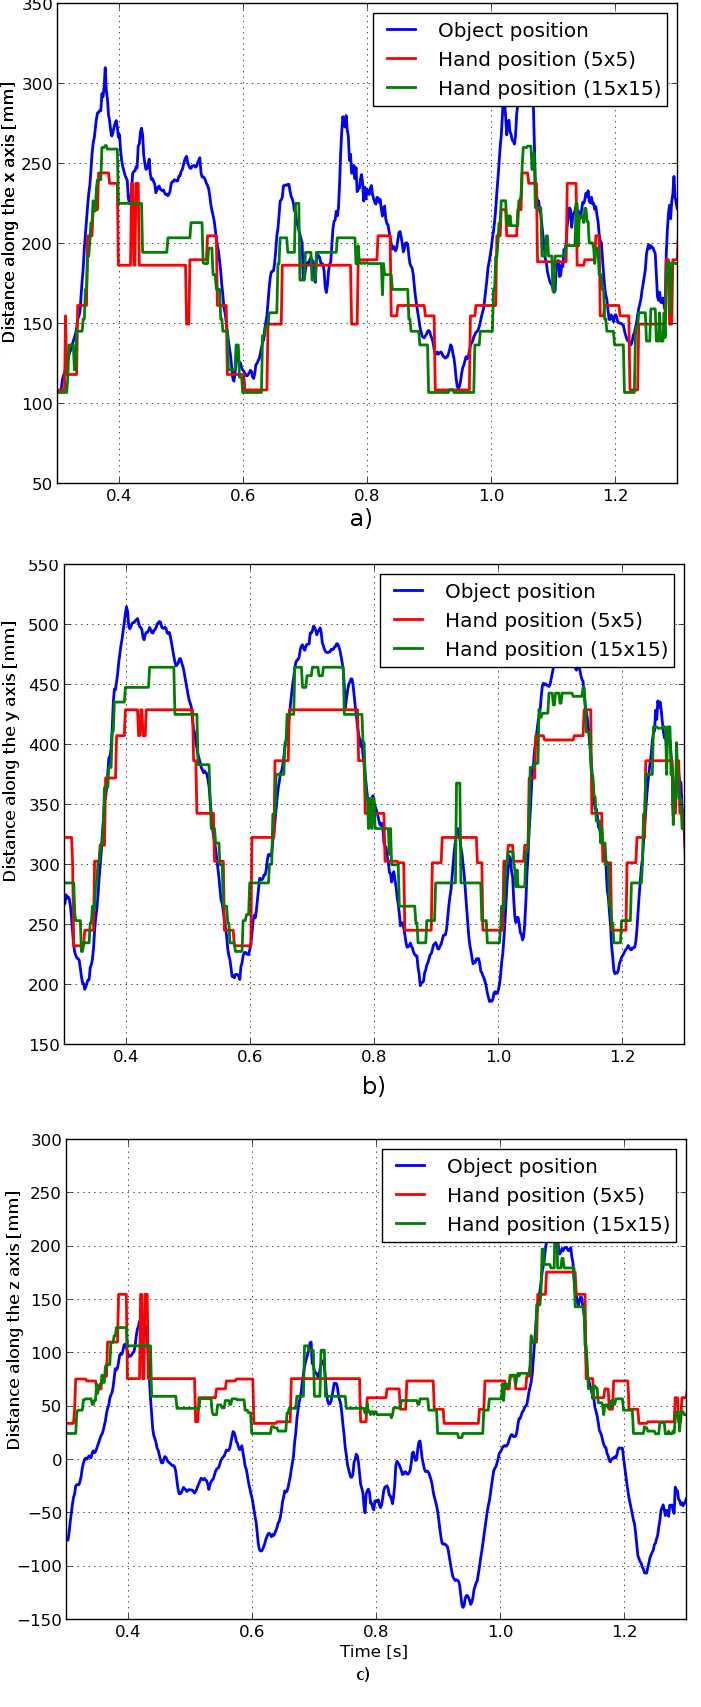
\epsfig{file=merged_trajectories_1.png, height=23cm}
\caption{Left hand trajectory along horizontal (a), vertical (b) and depth (c) axis as predicted by the two models and the ground truth value}
\label{lab:trajectory_x}
\end{figure}


% \begin{figure}[t]
% \centering
% \epsfig{file=trajectory_x1.png, height=8cm}
% \caption{Left hand trajectory along the horizontal axis as predicted by the two models and the ground truth value}
% \label{lab:trajectory_x}
% \end{figure}
% 
% \begin{figure}
% \centering
% \epsfig{file=trajectory_z1.png, height=8cm}
% \caption{Left hand trajectory along the vertical axis as predicted by the two models and the ground truth value}
% \label{lab:trajectory_y}
% \end{figure}
% 
% \begin{figure}
% \centering
% \epsfig{file=trajectory_y1.png, height=8cm}
% \caption{Left hand trajectory along the depth axis as predicted by the two models and the ground truth value}
% \label{lab:trajectory_z}
% \end{figure}

As a simple quantification measure of pointing we introduced the pointing precision error, which is defined as the Euclidean distance between the position of a marker and the hand position. A paired-samples t-test was conducted to compare precision errors for the $5\times 5$ network and the $15 \times 15$ network. There was a significant improvement in the performances from the $5 \times 5$ network ($Mean\ error=99.93mm$
, $Std.\ Dev.=32.10$) to the $15 \times 15$ network ($Mean\ error=80.32mm$, $Std.\ Dev.=33.41$) conditions; $t(1400)=76.47$, $p<0.05$. It is important to mention once again that the high error is the result of the difference between the maximal arm length and the unreachable object positions. 


\section{Implications of the Model}
With this work an important open question ``How can pointing emerge from grasping behaviour'' (T2.3 from \citep{Kaplan2006}) in developmental psychology and developmental robotics has been addressed. We identified and extended the informational and sensory prerequisites for realising pointing from motor babbling in a computational model. Compared to a similar model presented in \citep{SchillaciH11}, the advantage of our model is the biological plausibility, which aims to make a contribution towards the research in neuroscience and robotics. The modular organisation of the model in terms of sensory maps and associated representations of sensory data via Hebbian learning allows for easier extension and identification of its components with the biological equivalents. It has to be pointed out that the biologically inspired model has not been adopted just for the sake of reproducing a biological system into an artificial one. Rather, our aim is to provide the robot with capabilities such as autonomous learning, 
adaptability and plasticity. In fact, state-of-the-art robots still lack basic capabilities such as learning, adapting, reacting to unexpected circumstances, exhibiting a proper level of intelligence and autonomously and safely operating in unconstrained and uncertain environments.

Through the proposed SOM-model a robot can autonomously build up an internal representation of its body, or of parts of it. In particular, the nature of the proposed model allows an artificial agent to build up and, eventually, to reshape its internal body representation through the interaction with the external world.
In addition, a particular emphasis has been given to the developmental progression in the acquisition of motor and cognitive skills (such as attention manipulation through pointing gestures). We strongly believe that studying human development could give insights in finding those basic behavioural components that may allow for an autonomous mental and motor development in artificial agents. A robot capable of developing motor and mental skills autonomously can better deal with the aforementioned challenges related to real world scenarios.


Moreover, the results enable us to draw several parallels with respect to the development of pointing skills in infants. First, the two instances of the model can be compared to the two different stages of hand-eye coordination development. Under the assumption that the more advanced stage is described by more specialised neurons which facilitate pointing, the model containing more neurons simulates the later stage by performing significantly better in terms of smaller pointing errors. Second, we explored the influence of the data acquisition procedure through random motor babbling and showed that longer babbling phases yield better pointing accuracies. Following this line of arguments, one would expect that infants which explored a larger set of body configurations might acquire better manual coordination. This hypothesis can be further tested by analysing the motor coordination of children who were differently exposed to sports in their early childhood. 

When trained on different data, the model for pointing can be used for learning 
other sensorimotor skills. For example, one could use the model to learn 
relations between observed pointing gestures and motor commands for moving into 
the pointed direction, similarly to \citep{Bodiroza2013}. Knowing and handling 
these relations is important, as situations requiring them occur in everyday 
life. For example, in a bookstore when we point to a book on a shelf we cannot 
reach or on the street where we ask for an unknown path. Thus, for robots to 
exhibit human-like behaviour in such situations they need to be able to 
recognize the pointed position and to associate this position with a certain 
motor command which should be issued to reach that position. In order to achieve 
this behaviour, one would need to train one SOM to represent the space of joint 
configurations and associate this SOM with the motor commands in the second SOM. 
Depending on whether the robot should point or move, one should use one or the 
other 
SOM to guide the kinematics of the robot.



\chapter{Conclusion}
\label{chap:conclusion}


In the course of this work, a biologically inspired model of human acquisition of hand-eye coordination has been implemented in a robotic platform. 
Our aim was to follow a developmental paradigm by simulating the sensorimotor experience of an infant. Thus, prior to the interaction with a human the robot used body babbling to learn the extent of its own limb postures. After the acquisition of such a simple skill, a model based on self-organising maps has been trained and implemented in a robot. The robot exhibited pointing gestures when a human presented a tagged object in front of it, strengthening the hypothesis that pointing gestures might emerge from failed grasping actions. We showed that models containing more neurons account for a greater pointing precision. 
Although our model offers an extremely simplified representation of the complex neural networks observed in real biological systems, it sets up the ground for fastening the link between neuroscience and robotics. We believe that embodied intelligence emerging from simulated biological mechanisms is the key to creating truly intelligent machines. In addition, it might be useful to gain insights about the real neural systems. In particular, robots can be used to simulate behaviour of a young child interacting with the environment. We consider interaction essential for the development of social and cognitive skills. 
A purely theoretical approach to analysing development is not able to capture the abundance of sensory experience and interactions which contribute to brain plasticity and human development.


\section{Future Work}
\label{sec:future}

The research presented here can be expanded into multiple directions. 
To increase the pointing precision, one might like to address the training procedure in a greater detail and analyse the influence of learning parameters. The precision might also be improved by averaging the weight values over multiple winning neurons or simply by increasing the number of neurons in a network. 
More exciting questions with implications relevant for neuroscience might be tackled by increasing the level of biological realism in the model. This can be done by introducing more complex neuron models such as leaky integrate-and-fire or Hodgkin-Huxley that exhibit spiking behaviour. Using such models, one can implement learning rules which depend on spike timing and thus mimic biological systems more closely.

A mechanism which might reflect the ongoing development in neural models is the ability of a model to adapt to more complex inputs.
The adaptation should be observed as the increase in the model complexity which, in return, should be observable in the robot's behaviour. We speculate that one important aspect of such mechanism is captured by the increased number of neurons in the neural network.
Algorithms such as growing neural gas qualify as a starting point for simulation of such development. When using such a developmental paradigm in biologically plausible models, one should be able to draw parallels between the stages of development of the model and the stages of development in the biological system. The extension of this algorithm can include the batch learning mode, where the sensory data is processed in chunks. This allows for simultaneous exploration of environment and on-line adaptation of the model.

Within a PhD programme I will start upon receiving the Master's degree, I will continue to use biologically inspired models to investigate the development of higher cognitive functions. In particular, I will analyse sensorimotor and cognitive prerequisites for the emergence of creative and curious behaviour. I will explore the role of grounded cognition and associative relations in the retrieval of memory contents, and their influence on the creative behaviour.



\bibliography{literatur}
\bibliographystyle{apalike}

\cleardoublepage

\end{document}
